% Options for packages loaded elsewhere
\PassOptionsToPackage{unicode}{hyperref}
\PassOptionsToPackage{hyphens}{url}
\PassOptionsToPackage{dvipsnames,svgnames,x11names}{xcolor}
%
\documentclass[
]{article}
\usepackage{amsmath,amssymb}
\usepackage{iftex}
\ifPDFTeX
  \usepackage[T1]{fontenc}
  \usepackage[utf8]{inputenc}
  \usepackage{textcomp} % provide euro and other symbols
\else % if luatex or xetex
  \usepackage{unicode-math} % this also loads fontspec
  \defaultfontfeatures{Scale=MatchLowercase}
  \defaultfontfeatures[\rmfamily]{Ligatures=TeX,Scale=1}
\fi
\usepackage{lmodern}
\ifPDFTeX\else
  % xetex/luatex font selection
\fi
% Use upquote if available, for straight quotes in verbatim environments
\IfFileExists{upquote.sty}{\usepackage{upquote}}{}
\IfFileExists{microtype.sty}{% use microtype if available
  \usepackage[]{microtype}
  \UseMicrotypeSet[protrusion]{basicmath} % disable protrusion for tt fonts
}{}
\makeatletter
\@ifundefined{KOMAClassName}{% if non-KOMA class
  \IfFileExists{parskip.sty}{%
    \usepackage{parskip}
  }{% else
    \setlength{\parindent}{0pt}
    \setlength{\parskip}{6pt plus 2pt minus 1pt}}
}{% if KOMA class
  \KOMAoptions{parskip=half}}
\makeatother
\usepackage{xcolor}
\usepackage[margin=1in]{geometry}
\usepackage{longtable,booktabs,array}
\usepackage{calc} % for calculating minipage widths
% Correct order of tables after \paragraph or \subparagraph
\usepackage{etoolbox}
\makeatletter
\patchcmd\longtable{\par}{\if@noskipsec\mbox{}\fi\par}{}{}
\makeatother
% Allow footnotes in longtable head/foot
\IfFileExists{footnotehyper.sty}{\usepackage{footnotehyper}}{\usepackage{footnote}}
\makesavenoteenv{longtable}
\usepackage{graphicx}
\makeatletter
\def\maxwidth{\ifdim\Gin@nat@width>\linewidth\linewidth\else\Gin@nat@width\fi}
\def\maxheight{\ifdim\Gin@nat@height>\textheight\textheight\else\Gin@nat@height\fi}
\makeatother
% Scale images if necessary, so that they will not overflow the page
% margins by default, and it is still possible to overwrite the defaults
% using explicit options in \includegraphics[width, height, ...]{}
\setkeys{Gin}{width=\maxwidth,height=\maxheight,keepaspectratio}
% Set default figure placement to htbp
\makeatletter
\def\fps@figure{htbp}
\makeatother
\setlength{\emergencystretch}{3em} % prevent overfull lines
\providecommand{\tightlist}{%
  \setlength{\itemsep}{0pt}\setlength{\parskip}{0pt}}
\setcounter{secnumdepth}{5}
\usepackage{booktabs}
\usepackage{booktabs}
\usepackage{longtable}
\usepackage{array}
\usepackage{multirow}
\usepackage{wrapfig}
\usepackage{float}
\usepackage{colortbl}
\usepackage{pdflscape}
\usepackage{tabu}
\usepackage{threeparttable}
\usepackage{threeparttablex}
\usepackage[normalem]{ulem}
\usepackage{makecell}
\usepackage{xcolor}
\ifLuaTeX
  \usepackage{selnolig}  % disable illegal ligatures
\fi
\IfFileExists{bookmark.sty}{\usepackage{bookmark}}{\usepackage{hyperref}}
\IfFileExists{xurl.sty}{\usepackage{xurl}}{} % add URL line breaks if available
\urlstyle{same}
\hypersetup{
  pdftitle={Odd-Even Policy Evaluation on Pollution},
  pdfauthor={Traffic Boyz},
  colorlinks=true,
  linkcolor={Maroon},
  filecolor={Maroon},
  citecolor={Blue},
  urlcolor={blue},
  pdfcreator={LaTeX via pandoc}}

\title{Odd-Even Policy Evaluation on Pollution}
\author{Traffic Boyz}
\date{2024-01-09}

\begin{document}
\maketitle

\hypertarget{introduction}{%
\section{Introduction}\label{introduction}}

In recent years, the air quality problem has become a persistent problem
in DKI Jakarta. The air quality of the Indonesian capital has
deteriorated, with the PM2.5 average concentration escalating to 49.4
\texttt{\textbackslash{}mu}gram/m3 in 2019, which is about 66\% higher
than in 2017 (Zulkarnain et al, 2021). The deteriorating air quality
imposes other problems on the nation's capital, as air pollution has
been strongly linked to non-communicable diseases (NCDs), including
cardiovascular and chronic respiratory diseases and lung cancers, which
impose substantial burdens on the healthcare sector and the economy of
the country (Syuhada et al, 2023). In 2019, Jakarta witnessed NCDs
comprising 79\% (equivalent to 36,000 deaths) of the overall mortality
rate. The impact of air pollution in generating NCDs and premature
fatalities extends to significant consequences, including the loss of
productive labor, escalated healthcare expenses, a decline in the
country's gross domestic product (GDP), decreased productivity and
competitiveness of cities, and a deterioration in the overall quality of
life for residents. Recent findings from the World Bank revealed that
the annual cost of air pollution in Indonesia exceeded USD 220 billion
in 2019, constituting 6.6\% of the country's GDP (PPP).

Motor vehicles have become the primary source of pollution in DKI
Jakarta. In particular, the contribution of motor vehicles to the PM2.5
concentration of DKI Jakarta is approximately 32--57\%. This is due to
the rapid motorization of DKI Jakarta and its surrounding regions
(Zulkarnain et al, 2021). The rapid motorization in DKI Jakarta itself
is a problem that has existed for a long time, with the average annual
growth rate of motorized vehicles reaching 9.5 percent in 2017. In 1994,
the government introduced the 3-in-1 policy in an attempt to manage the
congestion on many main roads in DKI Jakarta. One of the latest policies
to be introduced, however, is the odd-even driving restrictions, a
traffic management system enacted to curtail the travel of passenger
cars on certain roads based on the vehicle license number. The odd-even
policy was initially implemented during the 2018 Asian Games and only
covered a small share of the main roads in Jakarta. Due to its perceived
success, it was expanded by the end of the event as a permanent policy
that covered the 9 main roads in DKI Jakarta. This policy is implemented
in the rush hour window of 6AM-10AM and 5PM to 10PM. The rationale of
the policy that only regulates the main roads is mainly because only
around 20 percent of trips in Jakarta were made with public
transportation, due in part to the lack of an integrated transportation
system for commuters (JakPost, 2021). The odd-even regulation, again,
was a success in terms of reducing congestion, as it again was expanded
into 16 more main roads, which therefore made the policy covering 25
main roads in DKI Jakarta. However, the impact of the regulation on air
quality remains in question, considering that there are many factors
that affect air quality. This brought the policy question of this paper:
how does Jakarta's odd-even traffic regulation policy affect the air
quality?

Several research studies have suggested that the implementation of
transportation demand management (TDM) through restrictions on vehicle
operations has demonstrated a reduction of pollutant emissions by over
50\% (Bigazzi and Rouleau, 2017). New Delhi, for example, has already
implemented the policy in 2016. The Energy Policy Institute at the
University of Chicago, in collaboration with Evidence for Policy Design,
conducted an analysis of the effects of the odd-even scheme implemented
in 2016. The study revealed that during the hours when the scheme was
enforced in January of that year, Delhi experienced a 14-16\% decrease
in PM2.5 levels. However, when the scheme was reintroduced in April of
the same year, there was no discernible reduction in pollution. This
paper aims to analyze in a similar way to what extent the odd-even
policy could affect the air quality, which we will also measure in PM2.5
levels.

The paper proceeds as follows. We begin by describing our data and
present why they are ~well suited to addressing the question of the
odd-even policy effect on the air quality in DKI Jakarta. We then
discuss our econometric model and describe in detail the various
instruments we use to address measurement errors. After we present our
main results and explore variations in our model assumptions, we discuss
the implications of our findings.

\hypertarget{background}{%
\section{Background}\label{background}}

The odd-even policy that we observed in this paper is the difference
between the odd-even policy in its initial expansion after the Asian
Games in 2018 and being enforced in December 2019, which covered 9 main
streets in DKI Jakarta, and the second expansion in September 2019,
which added 16 more streets being implemented the odd-even policy, thus
bring in total 25 streets covered by the policy. We refer to the DKI
Jakarta Governor's Regulation number 155-2018 and the DKI Jakarta
Governor's Regulation number 88-2019. We observed the change in these 2
time points, thus observing the monthly road data from April 2018 until
March 2020.

We used the odd-even policy as a treatment group in our paper, as we
wanted to observe the effect of the policy on our pollution. In choosing
our controlled group, we looked for roads with similarities to the roads
in the controlled group. Due to the limited availability of data on
traffic and exact origin-destination data, we used Jakarta's bus rapid
transit (BRT) system route as our proxy. Jakarta's BRT amounted to 15
million monthly passengers, with coverage of 85\% of DKI Jakarta,
serving as one of the biggest commuting services in DKI Jakarta. One of
the features of the BRT is the route is parallel with the most crowded
roads in Jakarta, therefore serving as a direct transportation
alternative to private vehicles. We proceeded to overlay the overlapping
BRT routes with the main roads in Jakarta, and the initial visualization
showed that it aligns with the roads that implement the odd-even policy.
Therefore, we used the roads that overlap with the BRT route as the
controlled roads in this research.

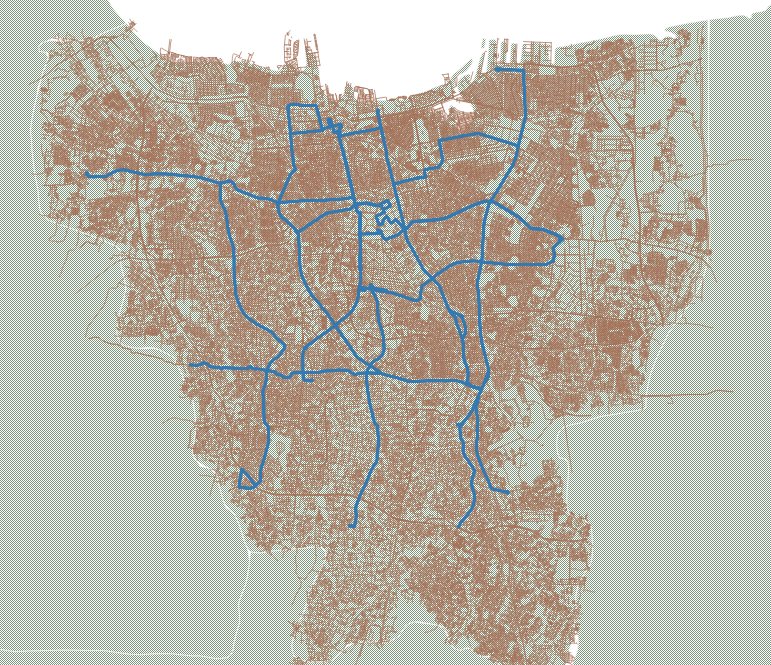
\includegraphics[width=0.5\textwidth,height=\textheight]{../Graph/control.png}
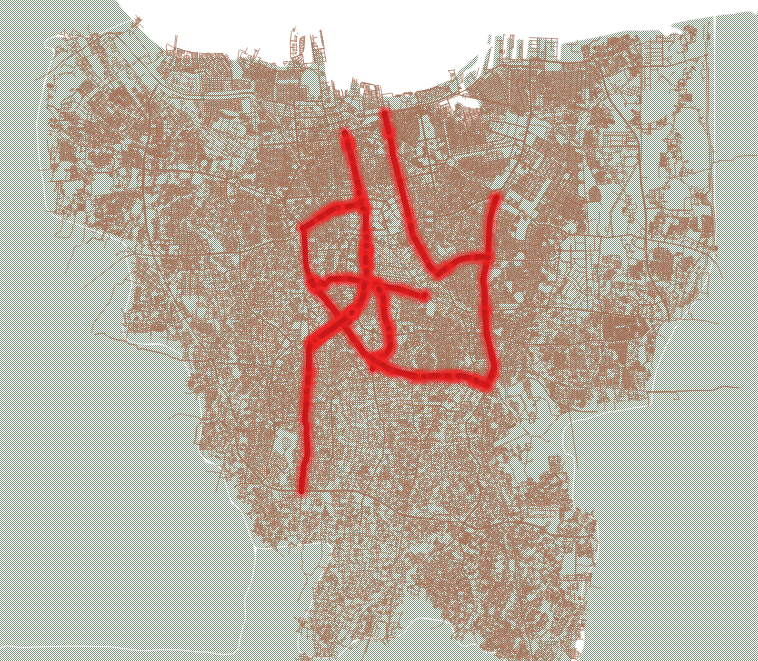
\includegraphics[width=0.5\textwidth,height=\textheight]{../Graph/gage.png}
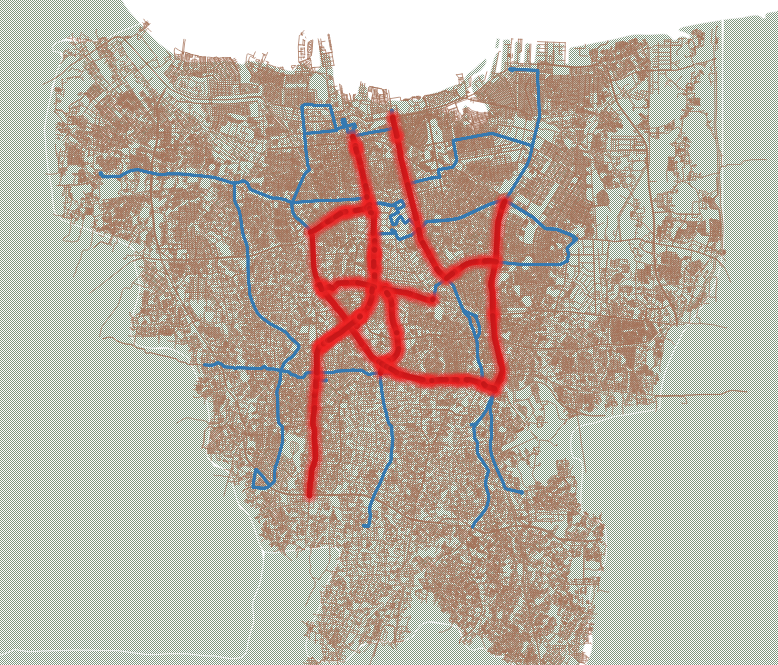
\includegraphics[width=0.5\textwidth,height=\textheight]{../Graph/overlay.png}

\hypertarget{data}{%
\section{Data}\label{data}}

\hypertarget{particulate-matter-2.5}{%
\subsection{Particulate Matter 2.5}\label{particulate-matter-2.5}}

The PM 2.5 data was obtained from the Van Donkelaar monthly average of
global particulate matter (2021). This data is generated using satellite
observation which has been calibrated using actual ground level
measurement, and modeled to to fill if there is any gap. The observation
unit of this data is coordinate grid with size of 0.01 x 0.01 degree,
which roughly equals to 1.1 x 1.1 km in Jakarta region. Ideally, there
are 1,113 satellite coordinate observations for every month across
Jakarta region, however in some cases when the cloud was thick enough to
prevent the satellite to measure, the data will be null. Some monthly
data are presented below.

\includegraphics{Rio_EDA_add-petatemp_files/figure-latex/unnamed-chunk-3-1.pdf}
\includegraphics{Rio_EDA_add-petatemp_files/figure-latex/unnamed-chunk-3-2.pdf}

\hypertarget{road}{%
\subsection{Road}\label{road}}

The road data were obtained from the Open Street Map. The road data were
then analyzed using the ArcGIS app, to assign a dummy value to signify
which road that implement the odd-even policy, which would be our
treatment road. The control roads were assigned to identify other roads
with similar traffic load as the comparison. This research uses primary
roads that contain bus rapid transportation (BRT) system route as the
control roads, because these roads should have similar characteristic as
the treatment roads.

There are 9 road groups that implement the odd-even policy
(\texttt{1\_hayam\_wuruk} to \texttt{9\_salemba}), while there is one
group of roads which do not implement the odd-even policy as the control
(\texttt{0\_not\_gage}). The location of each road can be seen in the
Background chapter.

\hypertarget{rainfall}{%
\subsection{Rainfall}\label{rainfall}}

Rainfall was obtained from Badan Pusat Statistik (BPS) Indonesia. This
data is the result of observation of Kemayoran weather station. Rain can
influence how long particulate matter emission can float in the air.
Increasing rainfall should be correlated to lower particulate matter
level. Rainfall as shown in the graph below (red line), has annual
seasonality characteristic, which tend to be high in the earlier of the
year (January - March) during the rainy season in Jakarta.

\includegraphics{Rio_EDA_add-petatemp_files/figure-latex/unnamed-chunk-4-1.pdf}

\hypertarget{holidays}{%
\subsection{Holidays}\label{holidays}}

Holidays data was obtained from various sources, such as from Indonesian
Cabinet Secretary office website. This data shows various national
holidays that happened and impacted the odd even policy in Indonesia.
There is one particular holiday which impact differently, which is the
Eid Al-Fitr holiday, because this holiday is particularly lengthy and
Jakarta population will go ``mudik'' or going to their hometown, which
usually located in smaller city throughout Indonesia. Therefore, Eid
Al-Fitr holiday, instead of increasing traffic in Jakarta, this holiday
would reduce traffic significantly. The distribution of the holidays
across period of interest can be seen in the table below.

\begin{table}

\caption{\label{tab:unnamed-chunk-5}Distribution of Mudik and Holidays across Period of Interest}
\centering
\begin{tabular}[t]{llrr}
\toprule
year & month & no\_working\_days & mudik\\
\midrule
2018 & 1 & 22 & 0\\
2018 & 2 & 19 & 0\\
2018 & 3 & 21 & 0\\
2018 & 4 & 21 & 0\\
2018 & 5 & 20 & 0\\
\addlinespace
2018 & 6 & 19 & 7\\
2018 & 7 & 22 & 0\\
2018 & 8 & 21 & 0\\
2018 & 9 & 19 & 0\\
2018 & 10 & 23 & 0\\
\addlinespace
2018 & 11 & 21 & 0\\
2018 & 12 & 19 & 0\\
2019 & 1 & 22 & 0\\
2019 & 2 & 19 & 0\\
2019 & 3 & 20 & 0\\
\addlinespace
2019 & 4 & 22 & 0\\
2019 & 5 & 21 & 0\\
2019 & 6 & 19 & 9\\
2019 & 7 & 23 & 0\\
2019 & 8 & 22 & 0\\
\addlinespace
2019 & 9 & 21 & 0\\
2019 & 10 & 23 & 0\\
2019 & 11 & 21 & 0\\
2019 & 12 & 20 & 0\\
2020 & 1 & 22 & 0\\
\addlinespace
2020 & 2 & 20 & 0\\
2020 & 3 & 20 & 0\\
\bottomrule
\end{tabular}
\end{table}

\hypertarget{exploratory-data-analysis}{%
\section{Exploratory Data Analysis}\label{exploratory-data-analysis}}

\hypertarget{seasonality-effect-on-pollution}{%
\subsection{Seasonality Effect on
Pollution}\label{seasonality-effect-on-pollution}}

In addition to rainfall, as discussed in the previous chapter, level of
particulate matter is also influenced by another weather event, such as
wind and humidity. However, due to limitation of usable data, month fix
effect is used instead. This approach should still be acceptable since
most of the weather characteristic period annually. This assumption is
proven by statistically significant regression of the month as dummy
variable (and rainfall) with robust standard error. The seasonality can
also be identified in the graph below. This regression result in
\texttt{r,\ summary\_eda2b\_bonth\_rain\$adj.r.squared} adjusted
R-squared.

\includegraphics{Rio_EDA_add-petatemp_files/figure-latex/unnamed-chunk-6-1.pdf}

\begin{longtable}[]{@{}lrrr@{}}
\caption{Regression Results of Controlling Seasonality and
Holidays}\tabularnewline
\toprule\noalign{}
& (1) & (2) & (3) \\
\midrule\noalign{}
\endfirsthead
\toprule\noalign{}
& (1) & (2) & (3) \\
\midrule\noalign{}
\endhead
\bottomrule\noalign{}
\endlastfoot
(Intercept) & 0.102*** & 0.148*** & 0.277*** \\
& (0.102) & (0.148) & (0.277) \\
month2 & 0.145*** & 0.210*** & 0.219*** \\
& (0.145) & (0.210) & (0.219) \\
month3 & 0.145*** & 0.210*** & 0.225*** \\
& (0.145) & (0.210) & (0.225) \\
month4 & 0.162*** & 0.210*** & 0.229*** \\
& (0.162) & (0.210) & (0.229) \\
month5 & 0.162*** & 0.210*** & 0.304*** \\
& (0.162) & (0.210) & (0.304) \\
month6 & 0.162*** & 0.210*** & 0.307*** \\
& (0.162) & (0.210) & (0.307) \\
month7 & 0.162*** & 0.210*** & 0.306*** \\
& (0.162) & (0.210) & (0.306) \\
month8 & 0.162*** & 0.210*** & 0.294*** \\
& (0.162) & (0.210) & (0.294) \\
month9 & 0.162*** & 0.210*** & 0.278*** \\
& (0.162) & (0.210) & (0.278) \\
month10 & 0.162*** & 0.210*** & 0.240*** \\
& (0.162) & (0.210) & (0.240) \\
month11 & 0.162*** & 0.210*** & 0.237*** \\
& (0.162) & (0.210) & (0.237) \\
month12 & 0.162*** & 0.210*** & 0.283*** \\
& (0.162) & (0.210) & (0.283) \\
year2019 & & 0.210*** & 0.205*** \\
& & (0.210) & (0.205) \\
year2020 & & 0.210*** & 0.228*** \\
& & (0.210) & (0.228) \\
month2 × year2019 & & 0.296*** & 0.344*** \\
& & (0.296) & (0.344) \\
month3 × year2019 & & 0.296*** & 0.285*** \\
& & (0.296) & (0.285) \\
month4 × year2019 & & 0.296*** & 0.289*** \\
& & (0.296) & (0.289) \\
month5 × year2019 & & 0.296*** & 0.289*** \\
& & (0.296) & (0.289) \\
month6 × year2019 & & 0.296 & 0.292*** \\
& & (0.296) & (0.292) \\
month7 × year2019 & & 0.296*** & 0.296*** \\
& & (0.296) & (0.296) \\
month8 × year2019 & & 0.296*** & 0.300*** \\
& & (0.296) & (0.300) \\
month9 × year2019 & & 0.296*** & 0.307** \\
& & (0.296) & (0.307) \\
month10 × year2019 & & 0.296*** & 0.332*** \\
& & (0.296) & (0.332) \\
month11 × year2019 & & 0.296*** & 0.316*** \\
& & (0.296) & (0.316) \\
month12 × year2019 & & 0.296*** & 0.307*** \\
& & (0.296) & (0.307) \\
month2 × year2020 & & 0.296*** & 0.407*** \\
& & (0.296) & (0.407) \\
month3 × year2020 & & 0.296*** & \\
& & (0.296) & \\
rainfall & & & 0.001*** \\
& & & (0.001) \\
Num.Obs. & 30051 & 30051 & 30051 \\
R2 & 0.763 & 0.835 & 0.835 \\
R2 Adj. & 0.763 & 0.835 & 0.835 \\
AIC & 192139.1 & 181356.1 & 181356.1 \\
BIC & 192247.1 & 181588.8 & 181588.8 \\
Log.Lik. & -96056.545 & -90650.029 & -90650.029 \\
F & 8799.842 & & \\
RMSE & 5.92 & 4.94 & 4.94 \\
\end{longtable}

\textbf{Note:} \^{}\^{} + p \textless{} 0.1, * p \textless{} 0.05, ** p
\textless{} 0.01, *** p \textless{} 0.001

\textbf{Note:} \^{}\^{} Robust standard errors are used

\hypertarget{near-analysis}{%
\subsection{Near Analysis}\label{near-analysis}}

This research main interest is to evaluate road level policy
implementation, however, since the pollution data uses coordinate
observation unit, each grid is assigned to the nearest road. This
assignment was done through Near Analysis geoprocessing in the ArcGIS
software. This analysis resulted in the nearest distance from all
observation coordinates to the selected roads.

Each observation coordinate is assigned with the nearest road and should
be less than 1,000 meters from it. This analysis can also be imagined as
identifying coordinates which located within 1,000 m buffer area from
the roads. If the distance from the nearest road is more than 1,000
meter, there will be no road assignment, and will be given null value.
The distribution of road to grid assignment is not equal, as shown in
the table below. From 1,113 observations, there are 888 coordinates
which are located more than 1,000 meters from any roads of interest.

\begin{table}

\caption{\label{tab:unnamed-chunk-9}Distribution of Coordinates to the Nearest Roads}
\centering
\begin{tabular}[t]{lr}
\toprule
nearest\_road & n\\
\midrule
0\_not\_gage & 162\\
1\_gajah\_mada & 3\\
2\_sudirman & 9\\
3\_fatmawati & 11\\
4\_tomang & 2\\
\addlinespace
5\_gatsu\_haryono & 16\\
6\_rasuna\_said & 3\\
7\_ahmad\_yani & 10\\
8\_pramuka & 3\\
9\_salemba & 6\\
\addlinespace
NA & 888\\
\bottomrule
\end{tabular}
\end{table}

\hypertarget{empirical-strategy}{%
\section{Empirical Strategy}\label{empirical-strategy}}

The odd-even policy motivates a straightforward fixed effect strategy
that estimates the causal effect of the policy and street pollution,
comparing average levels of air pollution across months-year. The
estimation equation is

\[
\small Y_{pm} = \beta_{1} S_{st}  + \mu_{s} + \tau_t + \varepsilon_{st}
\]

where \(\small Y_{pm}\) is the outcome of interest or the level of PM
2.5 in raster observed by road \(\_{s}\) and time \(\_t\);
\(\small S\_{st}\) is a binary variable indicating treatment status (the
odd-even policy), the road that implemented the policy becomes the
treatment group, while the control group is the street that never
implements the policy but still on a same level of characteristic. The
coefficient of interest is \(\beta\_{1}\), which represents the average
treatment effect between streets imposed with the odd-even policy and
not. \(\mu\_s\) represents street fixed effects that control for
time-invariant shocks common to all streets; \(\tau\*t\*\) represents
month-year fixed effects that control for time-varying shocks common to
all streets, and \(\varepsilon{st}\) is an idiosyncratic error term.

These estimates may still have a bias from the difference in time when
the policy was imposed because some roads implemented the policy in
August 2018, and the rest implemented the policy in September 2019. This
bias might threaten internal validity and affect the conclusion. The
event study research design can minimize this threat because it
estimates month by month effects relative to a base period
(Goodman-Bacon, 2018). Fo the next step, this study incorporates event
study into the estimation equation below.

\[
\tiny Y_{st} = 1\{\text{Odd-Even}\}[\sum_{y=-6}^{-2}\beta_{\text{pre}}\{t - t_s = y\} + \sum_{y=0}^{6}\beta_{\text{post}}\{t - t_s = y\}] + \mu_s + \tau_t + \varepsilon_{st}
\]

In the event study design, 1\{Odd Even Policy\} is a binary variable
identifying if a street is applied the odd-even policy, and \(t_s\) is
the month the policy was implemented. The coefficients of interest are
now \(\beta_{pre}\) and \(\beta_{post}\), which measure the effect
between the PM2.5 level and the odd-even policy in each of the 6 months
leading up to the policy and 6 months after.

\hypertarget{difference-in-the-control-and-treatment-group}{%
\subsection{Difference in the Control and Treatment
Group}\label{difference-in-the-control-and-treatment-group}}

Residuals is used for this analysis as a method to control the
seasonality effect based on previous analysis. Intuitively, this panel
data shows that most of the observed month, road that subject to odd
even policy, have higher unexplained pollution (residuals). The
difference are not very clear between the two groups in the scatter plot
below. The regression table proves that even though the treatment group
has higher unexplained pollution, the difference decreases after the
policy is implemented. This might be an indicator which shows the policy
is successful in decreasing the pollution in the observed grid. However,
since the implementation of the policy happened in two different time,
an event study approach needs to be implemented. Two dashed lines
represent two periods when the policy was implemented. Once in June 2018
and the other in September 2019.

\includegraphics{Rio_EDA_add-petatemp_files/figure-latex/unnamed-chunk-12-1.pdf}

\begin{longtable}[]{@{}lrr@{}}
\caption{Control and Treatment Difference Before and After
Policy}\tabularnewline
\toprule\noalign{}
& (1) & (2) \\
\midrule\noalign{}
\endfirsthead
\toprule\noalign{}
& (1) & (2) \\
\midrule\noalign{}
\endhead
\bottomrule\noalign{}
\endlastfoot
gage1 & 0.274*** & 0.207*** \\
& (0.274) & (0.207) \\
Num.Obs. & 1125 & 1575 \\
R2 & 0.012 & 0.015 \\
R2 Adj. & 0.011 & 0.015 \\
AIC & 6888.8 & 8725.8 \\
BIC & 6903.9 & 8741.9 \\
Log.Lik. & -3441.419 & -4359.885 \\
RMSE & 5.16 & 3.85 \\
Std.Errors & Custom & Custom \\
Before Policy & Yes & No \\
After Policy & No & Yes \\
\end{longtable}

\textbf{Note:} \^{}\^{} + p \textless{} 0.1, * p \textless{} 0.05, ** p
\textless{} 0.01, *** p \textless{} 0.001

\textbf{Note:} \^{}\^{} Robust standard errors are used

\hypertarget{event-study---two-way-fixed-effect}{%
\subsection{Event Study - Two Way Fixed
Effect}\label{event-study---two-way-fixed-effect}}

Before the event study approach, this study estimates the effect of the
odd-even policy in the table column (1). The coefficient shows that the
policy reduces the PM2.5 by 1.5 \(\mu\)gram/m3, on average, compared to
the road that did not implement the policy. After the event study was
conducted, the coefficient in column (2) got larger compared to the
previous estimate. This shows average PM2.5 decreases by 1.9
\(\mu\)gram/m3 in the Odd-even road. This is because the event study
minimizes the effect of unexpected factors between the first
implementation of the policy in August 2018 and September 2019 that
might reduce the magnitude of the policy. Finally, rainfall is
incorporated because this variable should have a high correlation with
PM2.5. However, column (3) shows that rainfall does not have a high
impact on pollution, and it is indicated by the coefficient of OD that
does not change.

\% Error: Argument `add.lines' must be NULL (default), or a list of
vectors.

The result of two way fixed effect using an event study is shown in the
chart below. The plot shows that the average PM2.5 decreased on the road
where the policy was implemented. However, a month later, the pollution
went back to the trend before the policy. Even though the coefficient of
Odd-event from the table above indicates that the average pollution was
reduced due to the policy, the behavior of monthly pollution bounced
back a month after the policy.

\includegraphics{Rio_EDA_add-petatemp_files/figure-latex/unnamed-chunk-18-1.pdf}

The plot of pollution residuals below also aligns with the finding of
``bounce back.'' This panel data shows that the unexplained pollution
(residuals) on the treated road was reduced after the policy was
implemented. This behavior was followed by the bounce back a month after
the policy.

\includegraphics{Rio_EDA_add-petatemp_files/figure-latex/unnamed-chunk-19-1.pdf}

\hypertarget{discussion}{%
\section{Discussion}\label{discussion}}

\hypertarget{policy-implication}{%
\subsection{Policy Implication}\label{policy-implication}}

This research found that the odd-even policy is statistically
significant in terms of reducing air pollution, controlling the
month-year, rainfall, roads, and the event study. However, the 1.9
coefficient means that the policy does not reduce the PM 2.5 level to a
high degree, which means the pollution level reduction of the policy is
low. However, it is still an effective policy to reduce air pollution,
given the statistically significant result. This implies that if there
are no other policy alternatives to reduce air pollution in the region,
the expansion of this policy to other major or crowded roads should be
considered. Another reason for the odd-even policy expansion is the
significant result that the observed roads in the controlled roads, in
which there is no implementation of the policy, have higher PM 2.5
levels compared to the treatment roads. Assuming that the exposure to
pollution is the same between the control and treatment roads, the
implementation of the odd-even policy in the control roads would have
benefitted the population that lives nearby.

Another significant policy implication is the result of the event study.
The result of the event study shows that the most significant reduction
in PM 2.5 level was only in the first month after the policy was
implemented. While the overall trend after the policy implementation
still shows a pollution reduction, it is not as high as the reduction in
the first month. There are a few possibilities for why the reduction in
the first month is the largest one. First, it is regarding the
enforcement issues. As with any other regulation that passed in the
region, the initial implementation always met with tight enforcement.
This yields the pollution reduction that is expected by the policy.
However, after some time, it is often that the enforcement becomes much
more loose. This is also the possible explanation for the case in New
Delhi, where the University of Chicago research team measured the PM 2.5
level for the odd-even policy, and found that during the first month of
the implementation it decreased by 14\%-16\%, but no significant
reduction in the reinstatement. Another possibility is that the people
adapted to the policy, either by switching to a motorcycle, as it is not
regulated by the odd-even policy, or by buying another car with a
different plate number. The latter, for one, could be explained in
further research as this study does not observe the actual number of
cars on the road with the odd-even policy implementation.~

The government also need take into consideration the cost of the policy,
as the odd-even restrictions on some roads limit the mobility of the
people, which, given that little transportation option is available,
could potentially harm the economic activities of the city. While the
debacle between the cost of limiting mobility and traffic congestion
remains, the implication of the policy is clear. The higher PM 2.5
levels in control roads, which are parallel to the BRT route signify
that the effect of public transport provision on the air quality is
still low. Expansion of the public transportation system is needed to
compensate for the limitation of mobility, should the government decide
to expand the odd-even policy to other major roads.~

It should also be noted that there are no differences between the PM 2.5
level of the observation whether the distance to the road is near or far
within the distance of 1000m. This means that the travel speed of PM 2.5
is high, therefore the benefit of the odd-even policy should be a
citywide benefit instead of only benefitting the people that live near
the road that implement the policy.

\hypertarget{conclusion}{%
\section{Conclusion}\label{conclusion}}

This study reinforces the argument that restrictions on vehicle
operations have demonstrated a reduction of pollutant emissions (Bigazzi
and Rouleau, 2017). The odd-even policy in DKI Jakarta did managed to
reduce the PM 2.5 level, albeit only in a small scale. The results also
consistent with the New Delhi case, which shows strongest effect in its
first month of implementation. It reflects the issues of enforcement of
the implementation, also the possibility of adaptation to the regulation
by the road users that reduce the efficacy of the policy, such as by
switching to motorcycles or buying another car with different plate
number. Finally, the policy is relevant to be expanded, considering
limited alternatives to reduce air pollution in DKI Jakarta.

\hypertarget{reference}{%
\section{Reference}\label{reference}}

Bigazzi, A., Rouleau, M. (2017).~ Can traffic management strategies
improve urban air quality? A review of the evidence. Journal of
Transport \& Health, p.~111-124,
\url{https://doi.org/10.1016/j.jth.2017.08.001}.

Goodman-Bacon, A., (2018). ``Public Insurance and Mortality: Evidence
from Medicaid Implementation,'' Journal of Political Economy, University
of Chicago Press, vol.~126(1), pages 216-262. DOI: 10.1086/695528

Syuhada G, Akbar A, Hardiawan D, Pun V, Darmawan A, Heryati SHA, Siregar
AYM, Kusuma RR, Driejana R, Ingole V, Kass D, Mehta S. (2023).~ Impacts
of Air Pollution on Health and Cost of Illness in Jakarta, Indonesia.
Int J Environ Res Public Health. Feb 7;20(4):2916. doi:
10.3390/ijerph20042916.~

Zulkarnain, A.G., (2021). Impact of odd-even driving restrictions on air
quality in Jakarta. International Journal of Technology. Volume 12(5),
pp.~925-934

Is Delhi's odd-even scheme to battle air pollution even effective?
(2023). Energy Policy Institute at the University of Chicago.
\url{https://epic.uchicago.edu/news/is-delhis-odd-even-scheme-to-battle-air-pollution-even-effective/}

What you need to know about Jakarta's odd-even traffic policy. (2023).
The Jakarta Post.
\url{https://www.thejakartapost.com/news/2018/04/23/what-you-need-to-know-about-jakartas-odd-even-traffic-policy.html}

\hypertarget{map-appendix}{%
\section{Map Appendix}\label{map-appendix}}

\includegraphics{Rio_EDA_add-petatemp_files/figure-latex/unnamed-chunk-21-1.pdf}
\includegraphics{Rio_EDA_add-petatemp_files/figure-latex/unnamed-chunk-21-2.pdf}
\includegraphics{Rio_EDA_add-petatemp_files/figure-latex/unnamed-chunk-21-3.pdf}

\end{document}
